\chapter{Requirements and approach}
\label{ch:requirements}

Turning a proof-of-concept into a platform that can actually be deployed means that the first step is to pin down what it has to do. Chapter~\ref{ch:introduction} framed the work around three objectives: architectural clarity~(O1), sensing quality~(O2), and operational reliability~(O3). This chapter translates those into six concrete, verifiable requirements. R1 operationalizes sensing quality (O2); R5 captures the architectural maintainability goal (O1); R3, R4, and R6 together address operational reliability (O3). R2 is a system constraint set by the deployment context — 20 simultaneous stations on a teaching budget — rather than derived from any single objective, and it applies across all three.

\section{Pedagogical requirements}

\textbf{Requirement 1:} The system should provide calibrated sensor data within uncertainty bounds small enough to support physiologically meaningful analysis. More specifically, VPD calculations that are traceable to reference instruments and spectral discrimination at the red/far-red band boundary.

\textbf{Design approach:} This asks the sensors to be able to resolve two things. One is the VPD gradient that drives stomatal response and the other is the red/far-red boundary that triggers phytochrome-mediated responses. Both of these require much more precision than what basic temperature/humidity or RGB sensors can provide (Figure~\ref{fig:vpd-calculation}). Chapter~\ref{ch:data-acquisition} works through the calibration method and the resulting uncertainty budgets.

\begin{figure}[H]
    \centering
    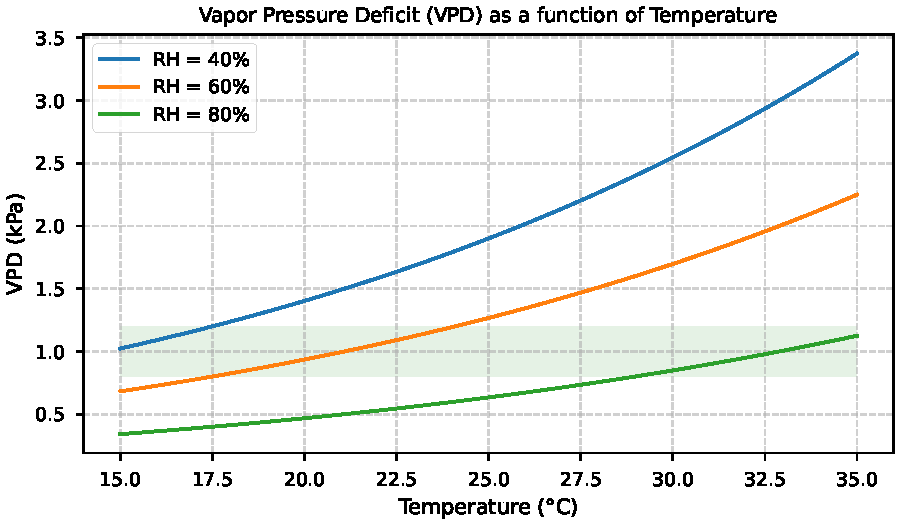
\includegraphics[width=0.85\textwidth]{Images/vpd_calculation}
    \caption[Temperature, Humidity, and Vapor Pressure Deficit]{The relationship between temperature, relative humidity, and the Vapor Pressure Deficit (VPD). Precise biological modeling of transpiration requires high-precision sensors because subtle errors in humidity translate to significant errors in VPD calculation, increasing at higher temperatures.}
    \label{fig:vpd-calculation}
\end{figure}

\section{Hardware and budget constraints}

\textbf{Requirement 2:} The total hardware cost per station should not exceed €150 as this enables simultaneous deployment of approximately 20 units within a teaching budget.

\textbf{Design approach:} The budget cap motivates each choice of component. Twenty groups each need a station at the same time, so each part has to earn its place on precision against cost. Commercial platforms can rely on more expensive industrial controllers where PhenoHive instead pairs a Raspberry Pi single-board computer with low-cost, I$^2$C-compatible sensors. I kept the Raspberry Pi over a cheaper microcontroller like an ESP32 because of the headroom. It can run a full Linux system, drive the high-resolution camera used for morphological tracking and manage a local persistence stack without needing to rely on a constant cloud connection.

Appendix~\ref{ch:appendix-bom} contains the full bill of materials. A unit comes to about €137 (Table~\ref{tab:bom}).


\section{Deployment context and operational resilience}

The stations are meant mainly for students' homes, but they should also work in a traditional greenhouse if need be. A home setting brings its own problems: power can get unplugged by accident, home Wi-Fi may be unstable or get reconfigured, and the surrounding environment is neither controlled nor steady.

\textbf{Requirement 3 (R3):} The system should not lose data during network outages and should recover connectivity autonomously, resuming data transmission without user intervention.

\textbf{Design approach:} The solution is an offline-first persistence model: measurements are written locally first and pushed to InfluxDB whenever it is reachable. When a push fails, the record is added to a local JSONL queue that replays on reconnection (Figure~\ref{fig:resilience-model}). Chapters~\ref{ch:storage} and~\ref{ch:evaluation} cover the design and the 48-hour disconnection test.

\textbf{Requirement 4 (R4):} First-boot setup should complete in under five minutes with no command-line interaction, so that students can begin collecting data immediately after connecting the device to Wi-Fi.

\textbf{Design approach:} On first boot, the \texttt{comitup} service broadcasts a temporary Wi-Fi hotspot. The student connects to it and enters the home network credentials through a captive portal in a web browser. The station then joins the network and starts pushing data automatically. Chapter~\ref{ch:evaluation} measures the end-to-end timing for each phase.

\begin{figure}[H]
\centering
\begin{tikzpicture}[
    node distance=0.8cm and 1.2cm,
    box/.style={draw, rounded corners, align=center, text width=2.8cm, minimum height=0.8cm, font=\footnotesize},
    fail/.style={draw=red!80, fill=red!5, dashed},
    success/.style={draw=green!80, fill=green!5, thick}
]
% Cloud-First
\node[font=\bfseries\footnotesize] (label1) at (2.2,1.2) {Standard Cloud-First Approach (Fragile)};
\node[box] (s1) at (0,0) {Sensor};
\node[box, right=of s1] (n1) {Network};
\node[box, right=of n1, fail] (db1) {Cloud Database\\(Data Loss)};
\draw[-{Latex}] (s1) -- (n1);
\draw[-{Latex}, red, dashed] (n1) -- (db1) node[midway, above, font=\tiny] {Outage};

% Local-First
\node[font=\bfseries\footnotesize] (label2) at (2.2,-1.2) {PhenoHive Local-First Approach (Resilient)};
\node[box] (s2) at (0,-2.5) {Sensor};
\node[box, right=of s2, success] (l2) {Local Archive\\(CSV / Queue)};
\node[box, right=of l2] (n2) {Network};
\node[box, right=of n2] (db2) {Cloud Database};

\draw[-{Latex}] (s2) -- (l2);
\draw[-{Latex}] (l2) -- (n2);
\draw[-{Latex}, dashed] (n2) -- (db2);
\node[below=0.1cm of l2, font=\tiny, text=green!60!black] {Authoritative / Buffer};
\end{tikzpicture}
\caption[Comparison of Data Persistence Strategies]{Two data-persistence strategies side by side. A standard cloud-first design is fragile because when the link to the cloud database drops during an outage, the readings in transit are lost. PhenoHive first writes to a local archive (CSV and queue) and treats it as authoritative, so an outage interrupts the upload and not the record.}
\label{fig:resilience-model}
\end{figure}

\section{Maintainability and handoff}

Teaching tools at a university change hands constantly so having a tightly coupled, monolithic codebase is a liability because a new TA who wants to add a sensor or change a setting has to touch the acquisition loop and can break it without realising.

\textbf{Requirement 5 (R5):} A new TA with no knowledge of the codebase should be able to add a new sensor and to modify a configuration value without having to modify the main core acquisition loop.

\textbf{Design approach:} The architecture has to be as modular and configuration-driven as possible. All of the sensor drivers, the core acquisition loop and the persistence therefore need to live each as distinct and testable components that can be changed, swapped out and tested one at a time.

\section{Data isolation and access control}

With 20 groups all writing to one central database at once, there is a real risk of data bleeding across groups. Each student should only be able to see and analyse their own station's data, so that their experimental hypotheses stay their own.

\textbf{Requirement 6 (R6):} Each student group should only have access to data from their own station. This should be enforced both on the Grafana permission layer and the InfluxDB query layer in order to maintain data integrity and isolation.

\textbf{Design approach:} A \texttt{station\_id} tag is added to the data at acquisition and stays with it throughout the whole pipeline. Grafana folder permissions and Flux queries filter each block cross-group access on their own. this makes it so that neither layer is a single point of failure. Chapter~\ref{ch:storage} covers the implementation.

\section{Requirements summary}

\begin{table}[htbp]
\centering
\caption[System-Level Requirements Summary]{Consolidated system-level requirements with traceability to the three objectives from Chapter~\ref{ch:introduction}: 1~architectural clarity, 2~sensing quality, 3~operational reliability. The verification column references the test or evidence that demonstrates compliance in Chapter~\ref{ch:evaluation}.}
\label{tab:requirements-summary}
\small
\setlength{\tabcolsep}{5pt}
\renewcommand{\arraystretch}{1.2}
\begin{tabularx}{\textwidth}{|P{0.8cm}|X|P{2.8cm}|P{1.1cm}|}
\hline
\textbf{ID} & \textbf{Requirement} & \textbf{Verification} & \textbf{Obj.} \\
\hline
R1 & Calibrated sensor data within research-grade uncertainty for VPD and spectral analysis & §\,\ref{sec:sht35-calibration}, §\,\ref{sec:tcs3448-calibration} & 2 \\
\hline
R2 & Total hardware cost $\leq$\,€150 per station & Appendix~\ref{ch:appendix-bom} & 1--3 \\
\hline
R3 & No data loss during network outages of $\geq$\,48\,h; full replay upon reconnection & 48\,h disconnection test (§\,\ref{ch:evaluation}) & 3 \\
\hline
R4 & First-boot setup in $<$\,5\,minutes with no command-line interaction & First-boot test (§\,\ref{ch:evaluation}) & 3 \\
\hline
R5 & New sensor addable without modifying the acquisition loop; configuration-driven extension & §\,\ref{ch:architecture} & 1 \\
\hline
R6 & Per-group data isolation enforced at both Grafana permission and InfluxDB query levels & Multi-station isolation test (§\,\ref{ch:evaluation}) & 3 \\
\hline
\end{tabularx}
\end{table}

